\clearpage{\pagestyle{empty}\cleardoublepage}

\chapter{Realizzazione e collaudo}

La cache \`e stata realizzata come componente indipendente, detto \texttt{Cache\_cmp}.\\
In questo capitolo saranno mostrate le caratteristiche principali di tale componente.

\section{Strutture dati}

Le strutture dati impiegate nel componente sono definite nel file \texttt{Cache\_lib.vhd}.

\lstset{language=VHDL, caption=Costanti e tipi di dato definiti nel file \texttt{Cache\_lib.vhd}, label=DescriptiveLabel, breaklines=true, basicstyle=\small, showspaces=false, showtabs=false, stringstyle=\ttfamily, showstringspaces=false,  tabsize=3} % basicstyle=\tiny\ttfamily}

\begin{lstlisting}

CONSTANT OFFSET_BIT : natural := 5;
CONSTANT INDEX_BIT : natural := 2;
CONSTANT TAG_BIT : natural := PARALLELISM - INDEX_BIT - OFFSET_BIT;
CONSTANT NWAY : natural := 2;

CONSTANT MESI_M : natural := 3;
CONSTANT MESI_E : natural := 2;
CONSTANT MESI_S : natural := 1;
CONSTANT MESI_I : natural := 0;

TYPE data_line IS ARRAY (0 to 2**OFFSET_BIT - 1) of STD_LOGIC_VECTOR (7 downto 0);

TYPE cache_line IS 
	RECORD
		data : data_line;
		status : natural;
		tag : STD_LOGIC_VECTOR (TAG_BIT-1 downto 0);
		lru_counter : natural;
	END RECORD;

TYPE set_ways IS ARRAY (0 to NWAY - 1) of cache_line;
		
TYPE cache_type IS ARRAY (natural range <>) of set_ways;
\end{lstlisting}


Il numero di bit di offset, indice e tag \`e stato parametrizzato per rendere pi\`u flessibile l'utilizzo del componente.

Sono stati inoltre definiti i seguenti tipi di dati:
\begin{itemize}
  \item \texttt{data\_line}: contiene i dati per una linea della cache, la cui dimensione \`e calcolata in base al numero di bit di offset;
  \item \texttt{cache\_line}: record contenente le informazioni su dati e stato di una linea;
  \item \texttt{set\_ways}: array di \texttt{NWAY} linee che compongono una via;
  \item \texttt{cache\_type}: array di vie, costituisce l'intera cache ??? (non so come scrivere... :S).
\end{itemize}

Per ogni \texttt{cache\_line} si tiene inoltre traccia di:
\begin{itemize}
  \item \texttt{data}: \texttt{data\_line} relativa alla linea corrente;
  \item \texttt{status}: indica lo stato MESI della linea;
  \item \texttt{tag}: bit dell'indirizzo che rappresentano il tag della linea;
  \item \texttt{lru\_counter}: contatore usato dalla politica di rimpiazzamento.
\end{itemize}


\begin{figure}[h!]
\centering
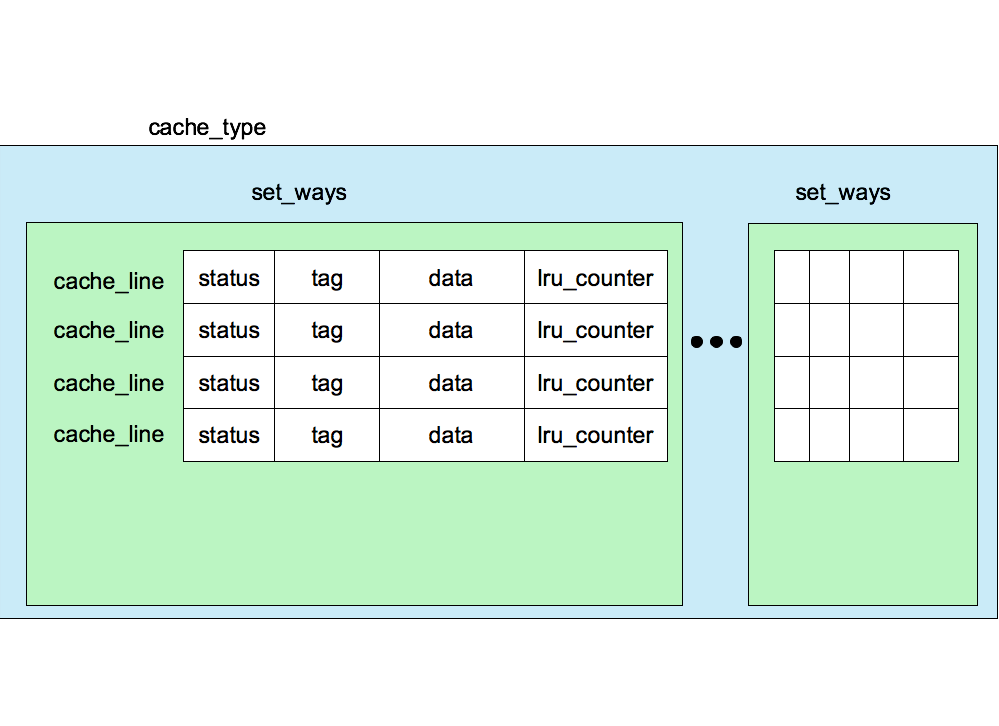
\includegraphics[width=\textwidth]{img/cacheType.png}
\caption{Schematizzazione delle strutture dati della cache}
\label{fig:c_type}
\end{figure}

In Fig. \ref{fig:c_type} \`e mostrata una schematizzazione delle strutture dati utilizzate all'interno del componente.

\section{Implementazione}

All'interno del componente \`e presente un unico process detto \texttt{cache\_process}, il quale risponde alle variazioni dei segnali di comando \texttt{ch\_reset}, \texttt{ch\_memrd}, \texttt{ch\_memwr}, \texttt{ch\_eads}.\\

All'interno del process vengono invocate le opportune procedure, tramite le quali si realizzano tutti i meccanismi per l'accesso e la modifica dei dati contenuti nella cache.\\


\lstset{caption=Codice VHDL del process \texttt{cache\_process}, label=DescriptiveLabel}

\begin{lstlisting}
cache_process: process (ch_reset, ch_memrd, ch_memwr, ch_eads) is
	variable word: STD_LOGIC_VECTOR (31 downto 0):= (others => '0');
	variable hit: STD_LOGIC;
	variable hit_m: STD_LOGIC;
begin
	if (ch_reset = '1') then -- reset
		ch_ready <= '0';
		cache_reset;
		-- Inizializzazione cache e ram per il debug			
		for i in 0 to 1023 loop
			RAM(i):= conv_std_logic_vector(i mod 256, 8);
		end loop;
	else
		if(ch_memrd = '1' and ch_memwr = '0') then -- memrd
			cache_read(word);
			ch_bdata_out <= word;
		elsif(ch_memrd = '0' and not ch_memwr'event and not ch_reset'event) then -- fine memrd
			ch_bdata_out <= (others => 'Z');
		end if;
				
		if(ch_memwr = '1' and ch_memrd = '0') then -- memwr
			word:= ch_bdata_in;
			cache_write(word);
		end if;
		
		if(ch_eads = '1') then -- snoop
			cache_snoop(hit, hit_m);
			ch_hit <= hit;
			ch_hitm <= hit_m;
		else
			ch_hit <= '0';
			ch_hitm <= '0';
		end if;
		
		ch_ready <= ch_memrd or ch_memwr;
			
	end if;
		
	ch_debug_cache <= cache;
end process cache_process;
\end{lstlisting}

Di seguito saranno brevemente descritte le procedure invocate all'interno del process.


\subsection{cache\_read} %(word: out)}

Parametri di output:
\begin{itemize}
  \item \texttt{word}: dato letto
\end{itemize}


Descrizione:
\begin{enumerate}
  \item Legge l'indirizzo dal bus separando index, tag e offset
  \item Verifica se c'\`e un hit attraverso \texttt{get\_way()}
  \item In caso di MISS applica la politica di rimpiazzamento richiamando \texttt{cache\_replace\_line()}
  \item Legge il dato dalla cache
  \item Aggiorna i contatori attraverso \texttt{cache\_hit\_on()}
  \item Pone il dato letto in \texttt{word} e lo restituisce 
\end{enumerate}	

\subsection{cache\_replace\_line} %(selected\_way: out)}

Parametri di output:
\begin{itemize}
  \item selected\_way: via sulla quale \`e stato caricato il dato rimpiazzato
\end{itemize}

Descrizione:
\begin{enumerate}
  \item Individua la linea da rimpiazzare, cio\`e quella con \texttt{lru\_counter} massimo
  \item Controlla se la linea ha stato MESI\_M e in tal caso ne fa il write-back invocando \texttt{ram\_write()}
  \item Carica il nuovo blocco nella cache sovrascrivendo il vecchio
  \item Modifica il bit di stato in base al valore di WT\_WB
  \item Restituisce il numero della via sulla quale \`e presente il dato appena caricato
\end{enumerate}
		

\subsection{cache\_hit\_on} %(hit\_index: in, hit\_way: in)}

Parametri di input:
\begin{enumerate}
  \item \texttt{hit\_index}: indice al quale si \`e verificato l'hit
  \item \texttt{hit\_way}: via nella quale si \`e verificato l'hit
\end{enumerate}

Descrizione:

Applica la politica di invecchiamento aggiornando i contatori, in particolare:
\begin{enumerate}
  \item incrementa i contatori di valore pi\`u basso della via corrente specificata da \texttt{hit\_way}
  \item resetta il contatore della via corrente
\end{enumerate}	

\subsection{cache\_inv\_on} %(inv\_index: in, inv\_way: in)}

Parametri di input:
\begin{itemize}
  \item \texttt{inv\_index}: indice da invalidare
  \item \texttt{inv\_way}: via da invalidare
\end{itemize}

Descrizione:

Applica la politica di invecchiamento aggiornando i contatori, in particolare:
\begin{enumerate}
  \item decrementa i contatori di valore pi\`u alto della via corrente specificata da \texttt{inv\_way}
  \item porta al valore massimo il contatore della via corrente
\end{enumerate}	
	

\subsection{cache\_write} %(word: in)}

Parametri di input:
\begin{itemize}
  \item \texttt{word}: parola ad scrivere nella cache

\end{itemize}

Descrizione:	
\begin{enumerate}
  \item Legge l'indirizzo dal bus separando index, tag e offset. 
  
  \item Verifica se c'\`e un hit attraverso \texttt{get\_way()}
  \item In caso di MISS applica la politica di rimpiazzamento richiamando \texttt{cache\_replace\_line()}
  \item Scrive il nuovo dato sulla cache
  \item Aggiorna i contatori attraverso \texttt{cache\_hit\_on()}
  \item Aggiorna il bit di stato ed esegue eventualmente il write-through.
\end{enumerate}
		


\subsection{get\_way} %(index: in, tag: in, way: out) }

Parametri di input:
\begin{enumerate}
  \item \texttt{index}: indice
  \item \texttt{tag}: tag da controllare
\end{enumerate}	

Parametri di output:
\begin{itemize}
  \item \texttt{way}: via nella quale \`e presente il dato
\end{itemize}

Descrizione:	
\begin{enumerate}
  \item Verifica se il dato \`e in cache, cio\`e se esiste una linea con tag uguale a quello specificato il cui stato \`e diverso da \texttt{MESI\_I}
  \item Se il dato non \`e presente restituisce way = -1
  \item Se il dato \`e presente restituisce il numero della via
\end{enumerate}
	
	
	
\subsection{ram\_write} %(tag, index, way)}

Parametri di input:
\begin{itemize}
  \item \texttt{tag}: tag della linea da scrivere
  \item \texttt{index}: index della linea da scrivere
  \item \texttt{way}: numero di via in cui si trova la linea da scrivere
\end{itemize}

Descrizione:
	1. Costruisce l'indirizzo del blocco a partire da \texttt{tag} e \texttt{index}
	2. Scrive i dati contenuti nel blocco sulla RAM
	

\subsection{snoop}
	Da dettagliare in seguito ????
	

\section{Diagrammi temporali}

\section{Problematiche principali affrontate}

(metteri anche tutti i problemi relativi al bus bidirezionale)\\

